\documentclass{article}
\PassOptionsToPackage{hyphens}{url}
\usepackage[dblblindworkshop, final]{neurips_2026}
\workshoptitle{The 6th Workshop on Mathematical Reasoning and AI}
\usepackage{fontspec}
\setmainfont{texgyretermes}[Extension=.otf,UprightFont=*-regular,
 BoldFont=*-bold,ItalicFont=*-italic,BoldItalicFont=*-bolditalic]
\setmonofont{Menlo}[Scale=MatchLowercase]
\usepackage{hyperref}
\usepackage{url}
\usepackage{booktabs}
\usepackage{amsfonts}
\usepackage{amsmath}
\usepackage{amssymb}
\usepackage{microtype}
\usepackage{graphicx}
\usepackage{adjustbox}
\usepackage{rotating}
\newcommand{\rot}[1]{\begin{sideways}#1\end{sideways}}
\hypersetup{hidelinks,pdftitle={The Errors Reviewers Catch: Statement-Level Autoformalization Errors and What Frontier Models Miss},pdfauthor={Alexander Korbonits}}
\title{The Errors Reviewers Catch:\\
Statement-Level Autoformalization Errors\\
and What Frontier Models Miss}
\author{Alexander Korbonits \\
Independent Researcher \\
\texttt{alexkorbonits@uchicago.edu}}
\begin{document}
\maketitle
\begin{abstract}
A formal statement can typecheck, be provable, and still fail to express the
intended informal mathematics. We study such statement-level errors in the
review history of a Lean~4 library of formalized open problems. From
squash-merged pull requests, we recover 74 natural negatives among 360
changed statements: semantic errors whose first pushed version differs from
the reviewer-approved version. All 360 are labeled by one annotator
against a 14-class error taxonomy, with the reviewers' corrections and
comments available. We evaluate twelve frontier models (eleven with
scoreable output) with and without those corrections. The highest agreement
with the reference labels is $F_1=0.79$ ($\kappa=0.73$) when corrections
and comments are supplied, versus $0.56$ ($\kappa=0.46$) for detection from the informal
statement and candidate formalization alone. Wrong carriers and definitional
mismatches are particularly difficult. Additional file context helps some
models but does not close the gap. Among complete-coverage models, the same detection prompt yields
$F_1=0.74$--$1.00$ on rule-written synthetic errors versus $0.29$--$0.52$
on natural errors restricted to rule-supported classes. The corpus of 5{,}726
documented statement pairs, the labeled negatives, model predictions, and evaluation code are publicly released.
\end{abstract}

\section{Introduction}
Autoformalization research measures whether models produce formal statements
that typecheck or admit proofs
\citep{wu2022autoformalization,azerbayev2023proofnet,ying2024leanworkbook}.
Whether those statements say what the informal source says is harder to
measure and often goes unmeasured, both in translation pipelines and in the
benchmarks built from them \citep{minif2f,tsoukalas2024putnambench}. Audits
have found statement defects in widely used formal benchmarks
\citep{ammanamanchi2026faults}. Faithfulness evaluation therefore
requires a separate comparison with the informal source: existing approaches
include reference-based equivalence checks \citep{poiroux2025reliable},
prover-based verification with vacuity filters \citep{zhou2024dont},
trained alignment scorers \citep{lu2024formalalign}, and LLM judges
\citep{zhang2026beyond}. Human-annotated formalization attempts already exist;
our contribution is to recover errors together with their corrections from
\emph{library review history}. For research-level mathematics, the working
detector remains human review.

We ask how well frontier models catch the errors human review catches, using
review history as the source of both errors and corrections. Our source is
\texttt{formal-conjectures}
\citep{firsching2026formalconjectures,formalconjectures2025}, an open-source
Lean~4 \citep{moura2021lean} library of formalized open problems, in which
every statement pairs a \LaTeX{} docstring (the informal side) with a Lean
declaration (the formal side) and passes human review before merge. Of 502
merged PRs, 33 contained a semantic statement error that review corrected
before merge. The resulting corpus contains
5{,}726 documented statement pairs and 74 labeled natural negatives.\footnote{Data,
predictions, and code are included in the supplementary snapshot; repository:
\url{https://github.com/korbonits/neurips-mathai-2026}.}
We compare model judgments with reference labels under two conditions:
\emph{assisted explanation}, which supplies the correction and review
comments, and \emph{detection}, which supplies only the informal--formal pair.
We also test whether file context or synthetic errors close the gap.

Software engineering draws similar distinctions: CodeReviewer separates
change-quality estimation, review-comment generation, and code refinement
\citep{li2022codereviewer}, and Toggle separates bug localization from repair
\citep{hossain2024toggle}. We draw the analogous line for formal statements,
between finding an error and explaining one when the fix is shown; we do not
claim that the resulting gap is specific to Lean.

\textbf{Contributions.} (1)~A corpus of 5{,}726 post-review (informal,
formal) statement pairs with full provenance, extracted with a parser
spot-checked by compilation. (2)~74 hand-labeled \emph{natural negatives}
mined from review history: real first-attempt formalization errors, each
paired with the reviewer-approved fix, inline review comments, and a 14-class
label. (3)~A 12-model, two-condition evaluation showing that
models agree with the reference labels substantially more often when the fix
is visible than when they must detect the error, with per-class analysis
locating the hardest cases in wrong carriers and definitional mismatches.

\section{A corpus of reviewed statement pairs}
\label{sec:corpus}
\textbf{Extraction.} We parse every top-level declaration in the library,
pairing each docstring with its statement (proof bodies stripped; definition
bodies retained, since for a definition the body is the content). A
compilation gate over sampled extractions passes 20/20. The tree at our
freeze commit yields 6{,}949 declarations, of which \textbf{5{,}726} carry
docstrings; each record retains file, line, and commit, status and
subject-class attributes where present, and citations found in the docstring.

\textbf{Mining corrections.} The repository squash-merges, so review history
is invisible on the main branch. We recover it: for each of 502 pull requests
merged between 29 May and 31 August 2026 (our shallow snapshot), we fetch the
PR branch head (\texttt{refs/pull/N/head}), locate the first pushed commit
past the merge base, and diff each declaration's statement text (not proof,
not docstring) against the merged result, restricted to files the squash
commit touched; the docstring at merge supplies the informal reference. For
the 124 force-pushed PRs, the platform's timeline recovers pre-push commits
for 18; 101 have garbage-collected commits, and five have no changes beyond
the merge base, so corrections already present in the earliest recoverable
version are missed.

\textbf{Reference labels and revision.} Mining yields 374 candidates, reduced
to 360 by deduplication and rename detection. The author labeled these using
a 14-class taxonomy, allowing multiple labels, with reviewer corrections and
528 inline comments available. Labels were assigned in two passes. A first pass, with model suggestions
visible, produced the 105 semantic errors of the reviewed submission. A
second, blind pass over all 360 candidates replaces it: model suggestions
and first-pass labels were hidden, and both formalizations were elaborated
in Lean where their difference was unclear. Forty-five first-pass errors became
controls and 14 controls became errors, leaving \textbf{74 semantic errors}
and 286 non-semantic changes; the latter are renames, API migrations, style
churn, and meaning-preserving rewrites. The final set has 93 semantic label assignments across 12 occupied classes
(Table~\ref{tab:classes}). Appendix~\ref{sec:labels} documents the transition and its limitations.
Figure~\ref{fig:example} shows a representative record.

\begin{figure}[t]\footnotesize
Docstring: \emph{Can the smallest modulus of a covering system be
arbitrarily large?}
\begin{verbatim}
theorem erdos_2 : answer(False) ↔                  -- first push
    ∃ B : ℕ, ∀ S, IsDistinctCoveringSystem S → minModulus S ≤ B

theorem erdos_2 : answer(False) ↔                  -- as merged
    ∀ B : ℕ, ∃ c : StrictCoveringSystem ℤ, ∀ i, ∃ m : ℕ,
      c.moduli i = Ideal.span {(m : ℤ)} ∧ B < m
\end{verbatim}
\caption{A natural negative (excerpt). The source docstring states that the
known answer is no. The \texttt{answer(False)} marker must pair with the
question's proposition (``can be arbitrarily large''), but the first push
paired it with the \emph{bounded} form, a double negation asserting the
opposite of the known result. It typechecks and reads plausibly; review
caught it. Reference labels: wrong-answer-marker, wrong-quantifier.}
\label{fig:example}
\end{figure}

\begin{table}[t]\centering\footnotesize
\begin{tabular}{@{}lp{0.66\textwidth}r@{}}
\toprule
error class & meaning & records \\
\midrule
    \textbf{wrong-type-or-domain} & wrong carrier: $\mathbb{N}$ vs $\mathbb{Z}$ vs $\mathbb{Q}$ vs $\mathbb{R}$, meaning-changing coercion & 20 \\
    \textbf{definitional-mismatch} & auxiliary definition does not capture the informal notion & 15 \\
    missing-hypothesis & informal side condition absent (positivity, distinctness, $n \ge 1$) & 12 \\
    \textbf{wrong-answer-marker} & \texttt{answer(True/False)} has incorrect polarity or wraps the wrong proposition & 11 \\
    \textbf{junk-value-trap} & meaning shifts through Lean junk values: $x/0$, $\mathbb{N}$ subtraction, $\inf\emptyset$ & 11 \\
    wrong-quantifier & $\exists/\forall$ swapped, wrong scope or order & 9 \\
    other & none of the above; explained in the record's note & 6 \\
    wrong-connective & $\wedge/\vee/\to/\leftrightarrow$ misuse, misplaced negation & 3 \\
    vacuous-or-trivial & trivially true or false (empty range, wrong index set) & 2 \\
    extraneous-hypothesis & formal statement assumes more than the informal one & 2 \\
    wrong-referent & points at the wrong declaration or constant & 1 \\
    wrong-constant-or-bound & off-by-one, wrong constant, strict vs non-strict inequality & 1 \\
\bottomrule
\end{tabular}

\caption{Error classes over the 74 natural negatives (multi-label). Wrong
carriers, definitional mismatches, and missing hypotheses dominate: errors of
\emph{semantics}, not syntax. Bold labels identify the Lean-semantics group
(Section~\ref{sec:eval}).}
\label{tab:classes}
\end{table}

\section{Can models catch what reviewers catch?}
\label{sec:eval}
We evaluate twelve models, eleven with scoreable output (four Claude-family
via the Anthropic API; GPT-5.6 Terra Pro, Gemini 3.1 Pro, Grok 4.6, Kimi K3,
DeepSeek V4 Pro, Qwen 3.8 Max, GLM 5.3, and Muse Spark 1.2 via OpenRouter),
using frozen prompts, initial chunks of 12 records,
and a 32k-token output budget; missing-response patches can use smaller batches. \textbf{Assisted}: the model sees the informal
statement, first formalization, reviewer-approved correction, up to six review comments, machine triage
bucket, and rename metadata. \textbf{Detection}: it sees only the informal statement and first
formalization.

Both conditions request labels and explanations, but scoring
measures binary semantic/non-semantic agreement (precision, recall, $F_1$,
and Cohen's $\kappa$ \citep{cohen1960kappa}) and class agreement, not the
correctness of explanations.

\begin{table}[t]\centering\small
\adjustbox{max width=\textwidth}{\begin{tabular}{lrrrrrrrrrr}
\toprule
 & \multicolumn{5}{c}{assisted} & \multicolumn{5}{c}{detection} \\
\cmidrule(lr){2-6}\cmidrule(lr){7-11}
model & $n$ & P & R & F1 & $\kappa$ & $n$ & P & R & F1 & $\kappa$ \\
\midrule
    Claude Haiku 4.5 & 360 & 0.42 & 0.93 & 0.58 & 0.41 & 360 & 0.24 & 0.45 & 0.31 & 0.06 \\
    Claude Sonnet 5 & 360 & 0.56 & 0.97 & 0.71 & 0.61 & 360 & 0.70 & 0.38 & 0.49 & 0.41 \\
    Claude Opus 5 & 360 & 0.63 & 0.97 & 0.77 & 0.69 & 360 & 0.67 & 0.30 & 0.41 & 0.33 \\
    Claude Fable 5 & 360 & 0.68 & 0.95 & 0.79 & 0.73 & 360 & 0.61 & 0.51 & 0.56 & 0.46 \\
    GPT-5.6 Terra Pro & 360 & 0.47 & 0.92 & 0.62 & 0.48 & 360 & 0.44 & 0.49 & 0.46 & 0.32 \\
    Gemini 3.1 Pro$^{\dagger}$ & 351 & 0.48 & 0.96 & 0.64 & 0.51 & 342 & 0.44 & 0.47 & 0.46 & 0.30 \\
    Kimi K3 & 360 & 0.66 & 0.85 & 0.75 & 0.67 & 360 & 0.54 & 0.45 & 0.49 & 0.37 \\
    Muse Spark 1.2 & 0 & -- & -- & -- & -- & 0 & -- & -- & -- & -- \\
    DeepSeek V4 Pro & 360 & 0.42 & 0.93 & 0.58 & 0.41 & 360 & 0.35 & 0.58 & 0.44 & 0.25 \\
    Qwen 3.8 Max$^{\dagger}$ & 328 & 0.46 & 0.97 & 0.62 & 0.49 & 335 & 0.42 & 0.55 & 0.48 & 0.33 \\
    Grok 4.6 & 360 & 0.53 & 0.95 & 0.68 & 0.56 & 360 & 0.40 & 0.57 & 0.47 & 0.30 \\
    GLM 5.3$^{\dagger}$ & 328 & 0.40 & 0.92 & 0.56 & 0.39 & 319 & 0.43 & 0.43 & 0.43 & 0.29 \\
\bottomrule
\end{tabular}
}
\caption{Agreement with the final reference on each condition's scoreable
records. Columns $n$ give answered counts; $\dagger$ marks models with
incomplete coverage in either condition. Bold marks the best value in each
column among complete-coverage models, ties included. Muse Spark 1.2 produced
no scoreable output within the output budget. Missing outputs are not counted
as correct or incorrect.}
\label{tab:main}
\end{table}

\textbf{Findings.} \emph{(i)} Every model with scored outputs in both
conditions drops from assisted to detection (Table~\ref{tab:main};
Figure~\ref{fig:comparison}). Claude Fable~5 leads both, falling from
$F_1=0.79$ to $0.56$, and the highest detection recall is $0.58$ (DeepSeek
V4 Pro). The gap survives the label revision: with predictions held fixed,
assisted $F_1$ exceeds detection $F_1$ for all eleven scoreable models under
both the submitted and final labels, by $0.18$--$0.44$ and $0.11$--$0.35$
respectively (Appendix~\ref{sec:labels}). \emph{(ii)} Models trade
precision for recall differently. Against a true error rate of 21\%, Claude
Opus~5 flags 9\% of records ($P=0.67$, $R=0.30$), while DeepSeek V4 Pro and
Claude Haiku~4.5 flag 33\% and 38\% at $P\le0.35$. \emph{(iii)} Per-class
recall locates the gap. We group wrong-type-or-domain, definitional-mismatch,
junk-value-trap, and wrong-answer-marker as the \emph{Lean-semantics group}
(57 label assignments). The best per-class counts are 5 of 20
wrong-type-or-domain errors, 4 of 15 definitional mismatches, 7 of 11
junk-value traps, and 6 of 11 answer-marker errors
(Table~\ref{tab:classrecall}); the surface-visible classes (wrong connective,
vacuous statements, wrong referent) are mostly caught, though with only one
to three examples each. \emph{(iv)} One model never produced scoreable output
and three only partially; staying within an output budget is part of the
reviewing task.


\begin{figure}[t]\centering
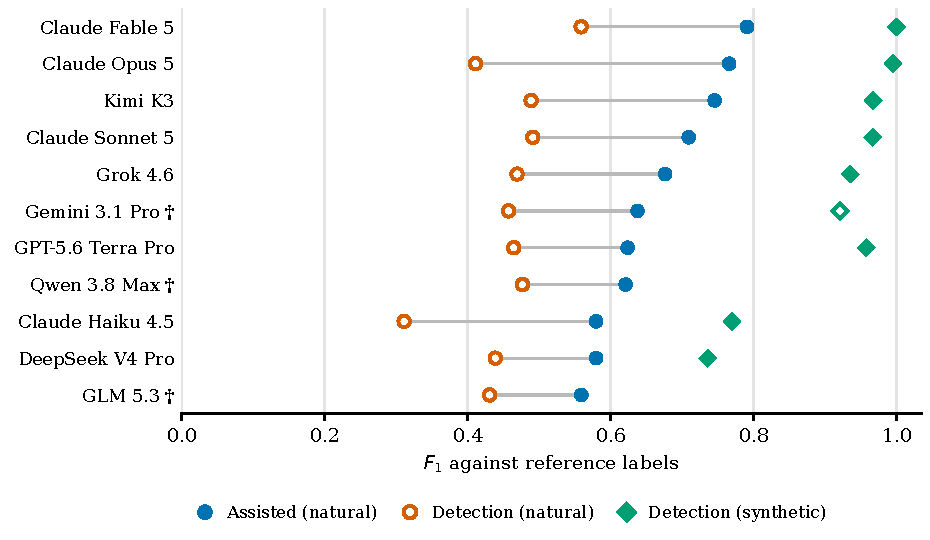
\includegraphics[width=0.82\linewidth]{figures/collapse.pdf}
\caption{Per-model $F_1$ with corrective information (assisted), without it
(detection), and on rule-written synthetic errors. Natural points use each
condition's answered records from the full 360-candidate set; $\dagger$ marks
incomplete natural coverage. Synthetic diamonds use a different population and
error prevalence; the hollow diamond marks Gemini's incomplete run (352 of 359
records). Qwen and GLM have too few synthetic responses to plot, and Muse has
no scored output. Table~\ref{tab:synthetic} gives the rule-supported natural
comparison.}
\label{fig:comparison}
\end{figure}

\section{What changes with context and synthetic errors?}
\label{sec:extensions}
\textbf{File context.} Seven models were rerun on detection with the
imports, namespace, and file-local auxiliary declarations (two dependency
hops) from each candidate's \emph{before} commit, plus hazard-oriented prompt
guidance; this tests context and guidance together and does not supply
Mathlib definitions. Detection $F_1$ changes by $-0.01$ to $+0.14$. Opus
gains most ($0.41\to0.55$, doubling its Lean-semantics recall from 8 to 16
of 57), but no augmented score exceeds the best unaugmented one
(Table~\ref{tab:context}; Appendix~\ref{sec:context}).

\textbf{Synthetic comparison.} We run the same detection prompt on 104
rule-written, typecheck-filtered perturbations of reviewed statements outside
the candidate set, with 255 unperturbed statements as controls. The rules
cover quantifier, carrier, hypothesis, and junk-value errors but not wrong
referents, definitional mismatches, or the catch-all class, so we compare
against natural records in rule-supported classes (339 records). Among models
answering every synthetic record, synthetic $F_1$ exceeds this natural
baseline by $0.35$--$0.60$ (Table~\ref{tab:synthetic}). Controls and error
prevalence differ between the two sets, but success on injected errors does
not predict performance on review-derived ones.

\begin{table}[t]\centering\small
\begin{tabular}{lrrrrr}
\toprule
 & \multicolumn{2}{c}{Natural, supported classes} & \multicolumn{2}{c}{Rule-written} & \\
\cmidrule(lr){2-3}\cmidrule(lr){4-5}
Model & $n$ & $F_1$ & $n$ & $F_1$ & $\Delta F_1$ \\
\midrule
Claude Haiku 4.5 & 339 & 0.29 & 359 & 0.77 & +0.48 \\
Claude Sonnet 5 & 339 & 0.45 & 359 & 0.97 & +0.51 \\
Claude Opus 5 & 339 & 0.40 & 359 & 1.00 & +0.60 \\
Claude Fable 5 & 339 & 0.52 & 359 & 1.00 & +0.48 \\
GPT-5.6 Terra Pro & 339 & 0.46 & 359 & 0.96 & +0.50 \\
Kimi K3 & 339 & 0.43 & 359 & 0.97 & +0.54 \\
DeepSeek V4 Pro & 339 & 0.39 & 359 & 0.74 & +0.35 \\
Grok 4.6 & 339 & 0.40 & 359 & 0.94 & +0.54 \\
\midrule
\multicolumn{6}{l}{\emph{Incomplete coverage: descriptive scores only}} \\
Gemini 3.1 Pro$^{\dagger}$ & 321 & 0.44 & 352 & 0.92 & +0.49 \\
GLM 5.3$^{\dagger}$ & 299 & 0.39 & 37 & 0.83 & +0.44 \\
\bottomrule
\end{tabular}
\caption{Detection on natural errors of rule-supported classes and rule-written
synthetic errors. Complete populations contain 339 and 359 records.
$\dagger$ marks incomplete coverage; GLM answered only 37 synthetic records.
Main-text ranges use complete rows. Qwen and Muse are omitted because neither
produced a scoreable synthetic response.}
\label{tab:synthetic}
\end{table}


\textbf{Intermediate assistance.} Removing review comments but keeping the
correction lowers assisted $F_1$ by only $0.04$--$0.08$ for seven models, so
the correction carries most of the signal. Oracle hints that an error exists,
or that name its class, raise class agreement but disclose the binary label,
so they do not measure detection; given a wrong class as a hint, models echo
it on 27 to 55 of roughly 74 errors (Appendix~\ref{sec:hints}).

\begin{table}[t]\centering\small
\adjustbox{max width=\textwidth}{\begin{tabular}{lrrrrrrrr}
\toprule
 & & detection & \multicolumn{3}{c}{context-augmented} & & \multicolumn{2}{c}{Lean-semantics recall} \\
\cmidrule(lr){3-3}\cmidrule(lr){4-6}\cmidrule(lr){8-9}
model & $n$ & F1 & P & R & F1 & $\Delta$F1 & detection & context-augmented \\
\midrule
    Claude Haiku 4.5 & 360 & 0.31 & 0.34 & 0.47 & 0.40 & $+0.09$ & 4/57 & 6/57 \\
    Claude Sonnet 5 & 360 & 0.49 & 0.71 & 0.43 & 0.54 & $+0.05$ & 8/57 & 11/57 \\
    Claude Opus 5 & 360 & 0.41 & 0.65 & 0.47 & 0.55 & $+0.14$ & 8/57 & 16/57 \\
    Claude Fable 5 & 360 & 0.56 & 0.55 & 0.55 & 0.55 & $0.00$ & 17/57 & 19/57 \\
    GPT-5.6 Terra Pro & 360 & 0.46 & 0.49 & 0.53 & 0.51 & $+0.04$ & 15/57 & 18/57 \\
    Kimi K3 & 360 & 0.49 & 0.45 & 0.50 & 0.47 & $-0.01$ & 14/57 & 17/57 \\
    Grok 4.6 & 360 & 0.47 & 0.43 & 0.55 & 0.48 & $+0.01$ & 17/57 & 20/57 \\
\bottomrule
\end{tabular}
}
\caption{Detection with file context versus unaugmented detection. All seven
context runs score 360 records. Pooled Lean-semantics recall counts correct
assignments in the Lean-semantics group defined in Section~\ref{sec:eval}.}
\label{tab:context}
\end{table}

\section{Discussion and limitations}
The errors that survive to review are errors of formal semantics: which
carrier a coercion lands in, what an auxiliary definition actually captures,
what a division by zero denotes. The classes that most require reasoning
about how a statement elaborates, wrong carriers and definitional mismatches,
are where models most often fail when working blind. Editorial checks in
formal-mathematics infrastructure, such as the Palomar
registry~\citep{tao2026palomar}, use a language model to judge whether a
formal statement faithfully renders its informal claim; our results bear on
such checks, though we do not evaluate that procedure. The highest detection
precision, $P=0.70$, suggests use for pre-review triage, but recall rules out
unsupervised gatekeeping, and deployed precision depends on the error rate.
Autoformalization systems should pair typechecking with semantics-aware
statement linting, such as junk-value analysis and counterexample search.
Evaluations that show the model a correction, as diff-explanation setups do,
overstate its reviewing ability.

\textbf{Limitations.} All data comes from one repository and one review
culture, and only merged pull requests with recoverable corrections enter.
The 111 declarations later changed by 69 fix-marked commits in the same
window show that some errors survive review; we do not label them. All
reference labels come from one annotator, who had earlier seen suggestions
from Claude Fable~5, the top model in both conditions; the blind pass hid
them, but prior exposure cannot be ruled out. Records cluster within pull requests, classes are
small, and results are single runs; chunk composition and routed providers,
which may serve quantized variants, may affect the scores. The library is
public and likely in training data; commit dates make contamination
auditable but do not rule it out.

\clearpage
\setlength{\bibhang}{1.6em}
\bibliographystyle{plainnat}
\bibliography{refs}
\clearpage
\appendix
\section{Reference-label revision and reproducibility}
\label{sec:labels}
The supplementary package includes the workshop data, predictions, prompts,
and code, alongside a current results summary. The same release is available at
\url{https://github.com/korbonits/neurips-mathai-2026}.
The final reference is stored under \texttt{artifact/data/}; the source records
file checksums in \texttt{artifact-version.json}, which the build verifies before
regenerating tables. The submitted 105-error labels are included separately
for the label-version sensitivity check.
Model runs were conducted in August--September 2026. Predictions that do not depend on reference labels were rescored
from disk after the blind pass. Hint prompts embed the reference class, so
hint runs were redone for records whose class changed.

For the label-version sensitivity check, we hold the current assisted and
detection predictions fixed and restrict each model to the intersection of
records answered in both conditions. We rescore these same records against
the submitted reference at artifact commit \texttt{478ffcc} and the final
reference. All eleven models retain higher assisted than detection $F_1$
under both references: the gaps range from $0.18$ to $0.44$ under the submitted
labels and from $0.11$ to $0.35$ under the final labels. The supplementary
robustness report gives per-model counts and scores; this checks sensitivity
to the label revision, not annotation correctness.

The first-pass subset check reported 23/40 binary self-agreement (57\%);
agreement with the model suggestion fell from 85\% to 62\% when it was
hidden. The blind pass agrees with the first pass on 301/360 binary judgments
($\kappa=0.57$), and on 273/360 exact class sets. The blind pass used more
Lean experience and elaboration of unclear cases, so this is not a
test--retest reliability estimate, and neither check substitutes for a second
annotator. The revised labeling treats omitting an \texttt{answer()} wrapper
or reversing equivalent sides of $\leftrightarrow$ as non-semantic.
The final reference supersedes the first-pass labels rather than averaging
the two passes. Of the 14 taxonomy options, non-semantic identifies controls,
informal-changed is unoccupied, and 12 semantic classes are represented.

Natural candidates retain the reviewer-approved version and comment evidence;
these support auditing the labels but do not prove faithfulness to the
informal source. The docstring is taken at merge, so matching that version
may differ from reconstructing the author's original intent. Eight candidates have no docstring (all are controls in the final reference);
the frozen prompt instructs the model to judge the remaining fields and note
this absence. They remain in the reported evaluation. Error directions
are available in the artifact but are not evaluated here. Supplementary files
include frozen prompts, final examples, and a description of score provenance.

\subsection*{LLM use disclosure}
LLM assistants were used for tooling, analysis code, and manuscript drafting
and revision; the author verified all claims, numbers, and citations. Claude
Fable~5 generated the initial labeling suggestions and is also an evaluated
model. The blind pass hid suggestions and prior labels,
but previous exposure and use of a single annotator remain limitations.
The camera-ready revision used an assistant to audit saved results, regenerate
tables, and revise the text. Model outputs are evaluated against human
reference labels; no claim of independent expert annotation is made.

\clearpage
\section{Class-level detection}
\label{sec:classresults}
\begin{table}[h]\centering\small
\adjustbox{max width=\textwidth}{\begin{tabular}{lrrrrrrrrrrr}
\toprule
error class (n) & \rot{Claude Haiku 4.5} & \rot{Claude Sonnet 5} & \rot{Claude Opus 5} & \rot{Claude Fable 5} & \rot{GPT-5.6 Terra Pro} & \rot{Gemini 3.1 Pro$^{\dagger}$} & \rot{Kimi K3} & \rot{DeepSeek V4 Pro} & \rot{Qwen 3.8 Max$^{\dagger}$} & \rot{Grok 4.6} & \rot{GLM 5.3$^{\dagger}$} \\
\midrule
    \textbf{wrong-type-or-domain} (20) & 0 & 2 & 2 & 2 & 4 & 4 & 2 & 1 & 4/15 & 5 & 2/16 \\
    \textbf{definitional-mismatch} (15) & 0 & 2 & 1 & 4 & 3 & 2 & 3 & 1 & 3/14 & 3 & 2/14 \\
    missing-hypothesis (12) & 5 & 6 & 5 & 8 & 7 & 5 & 4 & 5 & 8/11 & 5 & 3/9 \\
    \textbf{junk-value-trap} (11) & 2 & 3 & 3 & 6 & 5 & 3 & 5 & 2 & 7 & 3 & 4/10 \\
    \textbf{wrong-answer-marker} (11) & 2 & 1 & 2 & 5 & 3 & 5 & 4 & 6 & 5 & 6 & 3/8 \\
    wrong-quantifier (9) & 2 & 3 & 2 & 6 & 4 & 3 & 2 & 2 & 3/7 & 5 & 3/8 \\
    other (6) & 0 & 0 & 0 & 0 & 0 & 0 & 0 & 0 & 0 & 0 & 0 \\
    wrong-connective (3) & 3 & 1 & 1 & 1 & 2 & 1 & 1 & 2 & 2 & 1 & 1/2 \\
    extraneous-hypothesis (2) & 1 & 1 & 1 & 0 & 1 & 1 & 0 & 0 & 1 & 2 & 2 \\
    vacuous-or-trivial (2) & 0 & 2 & 2 & 2 & 1 & 1 & 2 & 0 & 2 & 2 & 1 \\
    wrong-constant-or-bound (1) & 0 & 1 & 1 & 1 & 1 & 1 & 1 & 0 & 1 & 1 & -- \\
    wrong-referent (1) & 1 & 1 & 1 & 1 & 1 & 1 & 1 & 1 & 1 & 1 & 1 \\
\bottomrule
\end{tabular}
}
\caption{Correct-class detection counts. Row totals count reference examples.
For incomplete models ($\dagger$), found/answered is shown when the answered
count is below the row total; a dash denotes no answered examples.
Bold labels identify the Lean-semantics group (Section~\ref{sec:eval}). Small
classes are descriptive only.}
\label{tab:classrecall}
\end{table}

Class recall requires assigning the correct class, not merely detecting that a statement contains some error.
No evaluated detector assigns the catch-all \texttt{other} label to any of
its six reference examples; this need not mean all six evade binary detection.

\section{Context and correction-only conditions}
\label{sec:context}

The context builder reads each file at its before commit and follows local
identifiers through two dependency hops. The declaration budget is 6,000
characters. Imports and namespace headers do not supply the definitions of
all imported names. The added instruction also points models to possible
semantic hazards, so effects cannot be attributed solely to extra code.

\begin{table}[h]\centering\small
\adjustbox{max width=\textwidth}{\begin{tabular}{lrrrrrrrr}
\toprule
 & & assisted & \multicolumn{3}{c}{correction only} & & \multicolumn{2}{c}{Lean-semantics recall} \\
\cmidrule(lr){3-3}\cmidrule(lr){4-6}\cmidrule(lr){8-9}
model & $n$ & F1 & P & R & F1 & $\Delta$F1 & assisted & correction only \\
\midrule
    Claude Haiku 4.5$^{\dagger}$ & 359 & 0.58 & 0.38 & 0.97 & 0.54 & $-0.04$ & 27/57 & 22/57 \\
    Claude Sonnet 5 & 360 & 0.71 & 0.48 & 0.97 & 0.64 & $-0.07$ & 38/57 & 37/57 \\
    Claude Opus 5 & 360 & 0.77 & 0.56 & 0.97 & 0.71 & $-0.05$ & 40/57 & 41/57 \\
    Claude Fable 5 & 360 & 0.79 & 0.59 & 0.95 & 0.73 & $-0.07$ & 41/57 & 35/57 \\
    GPT-5.6 Terra Pro & 360 & 0.62 & 0.38 & 0.96 & 0.54 & $-0.08$ & 40/57 & 43/57 \\
    Kimi K3 & 360 & 0.75 & 0.54 & 0.96 & 0.69 & $-0.06$ & 32/57 & 35/57 \\
    Grok 4.6 & 360 & 0.68 & 0.45 & 0.95 & 0.61 & $-0.07$ & 44/57 & 38/57 \\
\bottomrule
\end{tabular}
}
\caption{Keeping the corrected statement but removing review comments.
The correction-only condition retains other assisted metadata; $n$ gives
answered counts and $\dagger$ marks incomplete coverage. This intervention
is not a reviewer-comments-only condition.}
\end{table}
\clearpage
\section{Synthetic errors}
\label{sec:synthetic}
Each injected statement was typechecked in its original file. Typechecking
does not independently establish the intended semantic error or its class.
Rule transformations and their source records are recorded in
\texttt{scripts/make\_synthetic\_negatives.py} and
\texttt{data/negatives\_synthetic.jsonl} in the pinned artifact.
The natural comparison keeps controls and only semantic records whose labels
all occur in the rule-written set (339 records: 53 errors and 286 controls).
This matches class support, not frequencies, control construction, or error
prevalence. Partial-output runs are reported separately from complete ones;
missing predictions are not scored as successes or failures.

We do not evaluate specialized alignment scorers on these errors.

\section{Oracle hints and incorrect-hint compliance}
\label{sec:hints}
\begin{table}[h]\centering\small
\adjustbox{max width=\textwidth}{\begin{tabular}{lrrrrrrr}
\toprule
 & & \multicolumn{2}{c}{blind} & \multicolumn{2}{c}{error-present} & \multicolumn{2}{c}{class named} \\
\cmidrule(lr){3-4}\cmidrule(lr){5-6}\cmidrule(lr){7-8}
model & $n$ & class set & Lean-sem. & class set & Lean-sem. & class set & Lean-sem. \\
\midrule
    Claude Haiku 4.5$^{\dagger}$ & 359 & 0.52 & 4/57 & 0.82 & 17/57 & 0.92 & 48/57 \\
    Claude Sonnet 5$^{\dagger}$ & 293 & 0.79 & 5/45 & 0.84 & 14/45 & 0.98 & 44/45 \\
    Claude Opus 5$^{\dagger}$ & 285 & 0.83 & 4/35 & 0.87 & 17/35 & 0.94 & 34/35 \\
    Claude Fable 5$^{\dagger}$ & 253 & 0.78 & 12/43 & 0.85 & 17/43 & 0.92 & 41/43 \\
    GPT-5.6 Terra Pro & 360 & 0.71 & 15/57 & 0.82 & 26/57 & 0.92 & 51/57 \\
    Grok 4.6 & 360 & 0.66 & 17/57 & 0.83 & 26/57 & 0.92 & 50/57 \\
\bottomrule
\end{tabular}
}
\caption{Blind detection, an error-existence hint, and a class hint, on each
model's shared answered records ($n$); $\dagger$ marks incomplete coverage.
Both hints disclose the binary label.
Class-set agreement includes controls; pooled class recall uses reference
labels in the Lean-semantics group (Section~\ref{sec:eval}). Different row populations preclude
interpreting this as a model ranking.}
\end{table}
\begin{table}[h]\centering\small
\adjustbox{max width=\textwidth}{\begin{tabular}{lrrrr}
\toprule
 & controls & \multicolumn{2}{c}{errors, wrong class hinted} & errors, gold class hinted \\
\cmidrule(lr){2-2}\cmidrule(lr){3-4}\cmidrule(lr){5-5}
model & hint rejected & wrong class echoed & a gold class found & a gold class found \\
\midrule
    Claude Haiku 4.5 & 70/283 & 55/74 & 7/74 & 66/74 \\
    Claude Sonnet 5 & 33/243 & 50/74 & 11/74 & 72/74 \\
    Claude Opus 5 & 100/177 & 41/70 & 25/70 & 60/64 \\
    Claude Fable 5 & 73/90 & 40/73 & 26/73 & 67/74 \\
    GPT-5.6 Terra Pro & 184/286 & 27/74 & 26/74 & 61/74 \\
    Kimi K3 & 30/67 & 45/73 & 18/73 & 63/72 \\
    Grok 4.6 & 165/286 & 39/74 & 26/74 & 62/74 \\
\bottomrule
\end{tabular}
}
\caption{Wrong-hint control. Each record receives a class absent from its
reference label set. Denominators reflect available responses. Correct-hint
agreement can coexist with acceptance of incorrect labels.}
\end{table}
Hint runs were redone for records whose reference class changed. The
existence-hint condition remains incomplete for several models, so the first
table compares only shared answered records within each model. Kimi is omitted
from that comparison because its existence-hint responses have insufficient
coverage. Wrong-hint responses also have uneven coverage; they measure observed
compliance, not a population-wide failure rate. On controls, willingness to
accept a wrong-class hint varies widely: Claude Sonnet~5 rejects it on only
33 of 243, Claude Fable~5 on 73 of 90. Explanations were not independently
judged for correctness.

\end{document}
